\documentclass{beamer}
%
% Choose how your presentation looks.
%
% For more themes, color themes and font themes, see:
% http://deic.uab.es/~iblanes/beamer_gallery/index_by_theme.html
%
\mode<presentation>
{
  \usetheme{Warsaw}      % or try Darmstadt, Madrid, Warsaw, ...
  \usecolortheme{beaver} % or try albatross, beaver, crane, ...
  \usefonttheme{default}  % or try serif, structurebold, ...
  \setbeamertemplate{navigation symbols}{}
  \setbeamertemplate{caption}[numbered]
} 

%%%%%%%%%%%%%%%%%%%%%%%%
% ----- Packages ----- %
%%%%%%%%%%%%%%%%%%%%%%%%

\usepackage{lmodern}

% ----- AMS -----
\usepackage{amsmath}
\usepackage{amsfonts}
\usepackage{amssymb}

%\usepackage{amsthm} % Must come after amsmath.

\usepackage{mathtools}
\usepackage{dsfont}

\usepackage{graphicx}

%%%%%%%%%%%%%%%%%%%%%%%%
% ----- Commands ----- %
%%%%%%%%%%%%%%%%%%%%%%%%
\newcommand{\on}[1]{\operatorname{ \mathds{1}}_\text{$#1$} }

\newcommand{\inD}{\mathop{\overset{\mathrm{d}}{\longrightarrow}}}

\newcommand{\dist}[1]{\operatorname{#1}}
\newcommand{\iid}{\overset{\mathrm{iid}}{\sim}}


%\usepackage[english]{babel}
%\usepackage[utf8x]{inputenc}

\title[Frequency-Domain Bootstrap]{The Frequency-Domain Bootstrap of \\Dahlhaus \& Janas}
\author{Dmitriy Izyumin, Eugene Shvarts, Nick Ulle}
\institute{Final Project for Prof. Aue's STA 237A, Time Series Analysis}
\date{June 5, 2014}

\begin{document}

\begin{frame}[plain]
  \titlepage
\end{frame}

% Uncomment these lines for an automatically generated outline.
%\begin{frame}{Outline}
%  \tableofcontents
%\end{frame}

\section{Introduction}
%%%%%%%%%%%%%%%%%%%%%%%%%%%%%%%%%%%
%Dmitriy's Introduction section
%include subsections -- e.g., Ratio Statistics, Examples

\subsection{Bootstrapping and Time Series}
\begin{frame}{Bootstrapping and Time Series}

\begin{itemize}
\item Bootstrapping is based on resampling i.i.d. variables

\item How to deal with the dependence structure of time series?

\item Need (approximately) i.i.d. variables
\begin{itemize}
\item Time Domain: residuals, innovations
\item Frequency Domain: (Studentized) periodogram ordinates
\end{itemize}

\item Paper describes favorable properties of the latter

\end{itemize}
\end{frame}



\subsection{Spectral Mean}
\begin{frame}{Spectral Mean}
\begin{itemize}

\item $\phi = (\phi^{(1)},\cdots,\phi^{(d)})$, each $\phi^{(i)}$ of bounded variation

\item $I_T$ - tapered periodogram

\item Spectral mean $A(\phi, f) = \int_0^\pi \phi(\alpha)f(\alpha)d\alpha$

\item Canonical estimate $A(\phi,I_T) = \int_0^\pi \phi(\alpha)I_T(\alpha)d\alpha$

\end{itemize}
\end{frame}



\begin{frame}{Spectral Mean - Important Examples}
\begin{itemize}

\item Spectral mean $A(\phi, f) = \int_0^\pi \phi(\alpha)f(\alpha)d\alpha$

\item Autocovariance estimate $\hat{\gamma}(u), u \in \mathbb{Z}$\\
$\phi(\alpha) = 2\cos(\alpha u)$

\item Spectral distribution function estimate $\hat{F}_T(\lambda)$\\
$\phi(\alpha) = \on{[0,\lambda]}(\alpha)$

\end{itemize}
\end{frame}



\subsection{Ratio Statistics}
\begin{frame}{Ratio Statistics - Definition}
\begin{itemize}

\item Normalized spectral density: $g(\alpha)=\frac{f(\alpha)}{F(\pi)}$

\item Estimate: $J_T(\alpha)=\frac{I_T(\alpha)}{\hat{F}_T(\pi)}$

\item Ratio statistic: $A(\phi,J_T)=\frac{\int_0^\pi \phi(\alpha)I_T(\alpha)d\alpha}{\int_0^\pi I_T(\alpha)d\alpha} = \frac{A(\phi,I_T)}{A(1,I_T)}$

\end{itemize}
\end{frame}



\begin{frame}{Ratio Statistics - Important Examples}
\begin{itemize}
\item Ratio statistic: $A(\phi,J_T)=\frac{\int_0^\pi \phi(\alpha)I_T(\alpha)d\alpha}{\int_0^\pi I_T(\alpha)d\alpha} = \frac{A(\phi,I_T)}{A(1,I_T)}$


\item Autocorrelation estimate $\hat{\rho}_T(u), u \in \mathbb{Z}$\\
$\phi(\alpha)=\cos(\alpha u)$

\item Normalized sdf estimate $\hat{F}_T(\lambda) / \hat{F}_T(\pi)$\\
$\phi(\alpha) = \on{[0,\lambda]}(\alpha)$

\end{itemize}
\end{frame}



\begin{frame}{Whittle Estimators}
\begin{itemize}

\item Parametric family of spectral densities: $\mathcal{F}=\{f_\theta: \theta \in \Theta\}, \Theta \in \mathbb{R}$

\item Whittle's likelihood: $\mathcal{L}_T(\theta) = \frac{1}{2\pi}\int_0^\pi \left[ \log f_\theta (\alpha) + \frac{I_T(\alpha)}{f_\theta(\alpha)} \right]d\alpha$

\item $\hat{\theta}$ obtained by minimizing $\mathcal{L}_T(\theta)$

\item Spectral mean with $\phi(\alpha) = \nabla \frac{1}{f_\theta}(\alpha)$

\end{itemize}
\end{frame}
 		%uncomment this line to insert your slides
%%%%%%%%%%%%%%%%%%%%%%%%%%%%%%%%%%%

\section{The Bootstrap Approximation}
%%%%%%%%%%%%%%%%%%%%%%%%%%%%%%%%%%%
%Eugene's The Bootstrap Approximation section
%include subsections -- e.g., Algorithm, Assumptions, Validity
% \subsection{Bootstrap Periodogram}
 
 \begin{frame}{Spectral Mean Distribution}
If we were to Studentize our periodogram values $\{I_j\}$ with estimated spectral density $\hat f$ in order to obtain bootstrap values $\{I_j^*\}$, we could form the bootstrap approximation 
$$
B(\phi,I_T^*) := \frac{\pi}{n} \sum_{j=1}^n \phi_j I_j^*~~\text{, where}~~\phi_j := \phi(2\pi j/T)~~.
$$ \pause

Under appropriate conditions ...
 \begin{itemize}
 \item $\sqrt T \bigl( A(\phi,I_T) - A(\phi,f)\bigr)$ is asymptotically normal with variance $=~~2\pi \int \phi^2 f^2 + (\kappa_4 / \sigma^4)\left(\int \phi f\right)^2~$.
 \item $\sqrt T \bigl( B(\phi,I_T^*) - B(\phi,\hat f)\bigr)$ is asymptotically normal with variance $\propto~~2\pi \int \phi^2 f^2~$.
 \pause
 \end{itemize}
 For ratio statistics, second term vanishes!
 \end{frame}
 
 \begin{frame}{Algorithm}
 Let $n = \lceil T/2\rceil$ and $I_j := I_T(2\pi j/T)$. 
 \begin{enumerate}
 \item Obtain periodogram sample values $\{I_j\},~ j=1:n$.
 \item Obtain estimate $\hat f$ of spectral density $f$ (e.g., kernel estimate).
\pause
 \item Obtain Studentized periodogram samples $\hat\epsilon_j := I_j / \hat f_j$.
 \item Rescale the $\hat\epsilon_j$'s by their mean, so that $\tilde\epsilon_j := \hat\epsilon_j / \{(1/n) \sum_j \hat\epsilon_j\}$.
 \pause
 \item Sample the empirical distribution of $\{\tilde\epsilon_j\}$ to obtain a bootstrap sample $\{\epsilon^*_j\}$ (whose size may differ from $n$).
 \item Define bootstrap periodogram values via $I_j^* := \hat f_j \epsilon^*_j$.
 
 \end{enumerate}
 \end{frame}

 \subsection{Validity}
 
 \begin{frame}{Some Assumptions}
 Performance guarantee of the bootstrap approximation requires ...
 \begin{itemize}
 \item $\{X_t:t\in\mathbb Z\}$ is a real-valued linear process: $X_t = \sum_{u\in\mathbb Z} a_u \xi_{t-u}$ The $\{\xi_t\}$ satisfy $\mathbb E \xi_1 = 0$, $\mathbb E \xi_1^2 = 1$, $\mathbb E \xi_1^8 <\infty$, $\mathbb E \xi_t^3 = 0$. \\ The $\{a_t\}$ satisfy $\sum_t t^2 |a_t| < \infty$.
 \item $\sup_{\alpha\in[0,\pi]} |\hat f(\alpha) - f(\alpha)| \to 0$ almost surely.
 \item $\phi$ is a $d$-dimensional vector of BV functions $\phi^{(r)}:[0,\pi]\to\mathbb R$, each with even periodic extension to all of $\mathbb R$. 
 \item The taper $h_t$ has the form $h_t := h(t/T)$, with $h:\mathbb R\to[0,1]$ a BV function with support in $(0,1]$.
 \end{itemize}
 \end{frame}
 
 \begin{frame}{More Technical Assumptions}
Edgeworth expansions are used to show that we outperform the normal approximation. For these we need  ...
 \begin{itemize}
\item  The $\{a_t\}$ and Fourier coefficients $\{\hat\phi (\omega)\}$ vanish exponentially. That is, for a fixed $\tau \in (0,1)$, $|a_t| \le \tau^{|t|}$ and $\|\hat\phi(\omega)\| \le \tau^{|\omega|}$.
\item several other detailed technical assumptions on $h$, $\xi$, and $\phi$ (more than five minutes allow! See the paper).
 \end{itemize}
 \end{frame}
 
\begin{frame}{Convergence Rate}
\only<1>{
\begin{itemize}
\item To bootstrap the distribution of $A(\phi,J_T)-A(\phi,g)$, use the statistic $B(\phi,J_T^*)-B(\phi,\hat g)$, where $\hat g_j := \hat f_j / \{(\pi/n) \sum_k \hat f_k\}$.
\item Let $D_T^2 = V_T^{-1}$, where $V_T$ is the covariance matrix of $\sqrt T A(\phi,J_T)$. Define $\hat D_T$ analogously via $\sqrt T B(\phi,J_T^*)$.
\item Let $P^*$ denote the conditional distribution given the data.
\end{itemize} }

\begin{block}{Theorem}
Suppose the assumptions stated in the paper hold. Then for almost all samples $\{I_j\}$, 
$$
\sup_C \left| P\bigl( \sqrt T D_T(A(\phi,J_T) - A(\phi,g)) \in C \bigr) \right. - $$ $$
\left. P^*\bigl(\sqrt T \hat D_T(B(\phi,J_T^*)-B(\phi,\hat g)) \in C  \bigr)\right| = o(T^{-1/2})~~.
$$
The $\sup$ is taken over convex measurable subsets of $\mathbb R^d$. 
\end{block}

\uncover<2>{
In short, estimating the distribution of the standardized spectral density by resampling from the standardized periodogram is consistent, and the convergence rate is asymptotically better than that achieved by the normal approximation. 
}
\end{frame} 
 
  		%uncomment this line to insert your slides
%%%%%%%%%%%%%%%%%%%%%%%%%%%%%%%%%%%

\section{Empirical Examples}
%%%%%%%%%%%%%%%%%%%%%%%%%%%%%%%%%%%
%Nick's Numerical Experiments section
%include subsections -- e.g., Reproduced Simulations, Estimation of ___, Discussion, ...

\begin{frame}{Simulation Example}
Simulate the $\textrm{AR}(1)$ process $X_t = 0.9 X_{t-1} + Z_t$.
\begin{itemize}
    \item
    Innovations $\{Z_t\} \iid \dist{U}(-\sqrt{3}, \sqrt{3})$ are
    mean 0, variance 1 white noise.

    \item
    Draw $64$ observations.

    \item
    Recall that $\hat{\rho}(1)$ is the Yule-Walker estimate for the
    AR parameter~$0.9$.

\end{itemize}
\end{frame}

\begin{frame}{Series Plot}
    \begin{figure}
    \centering
    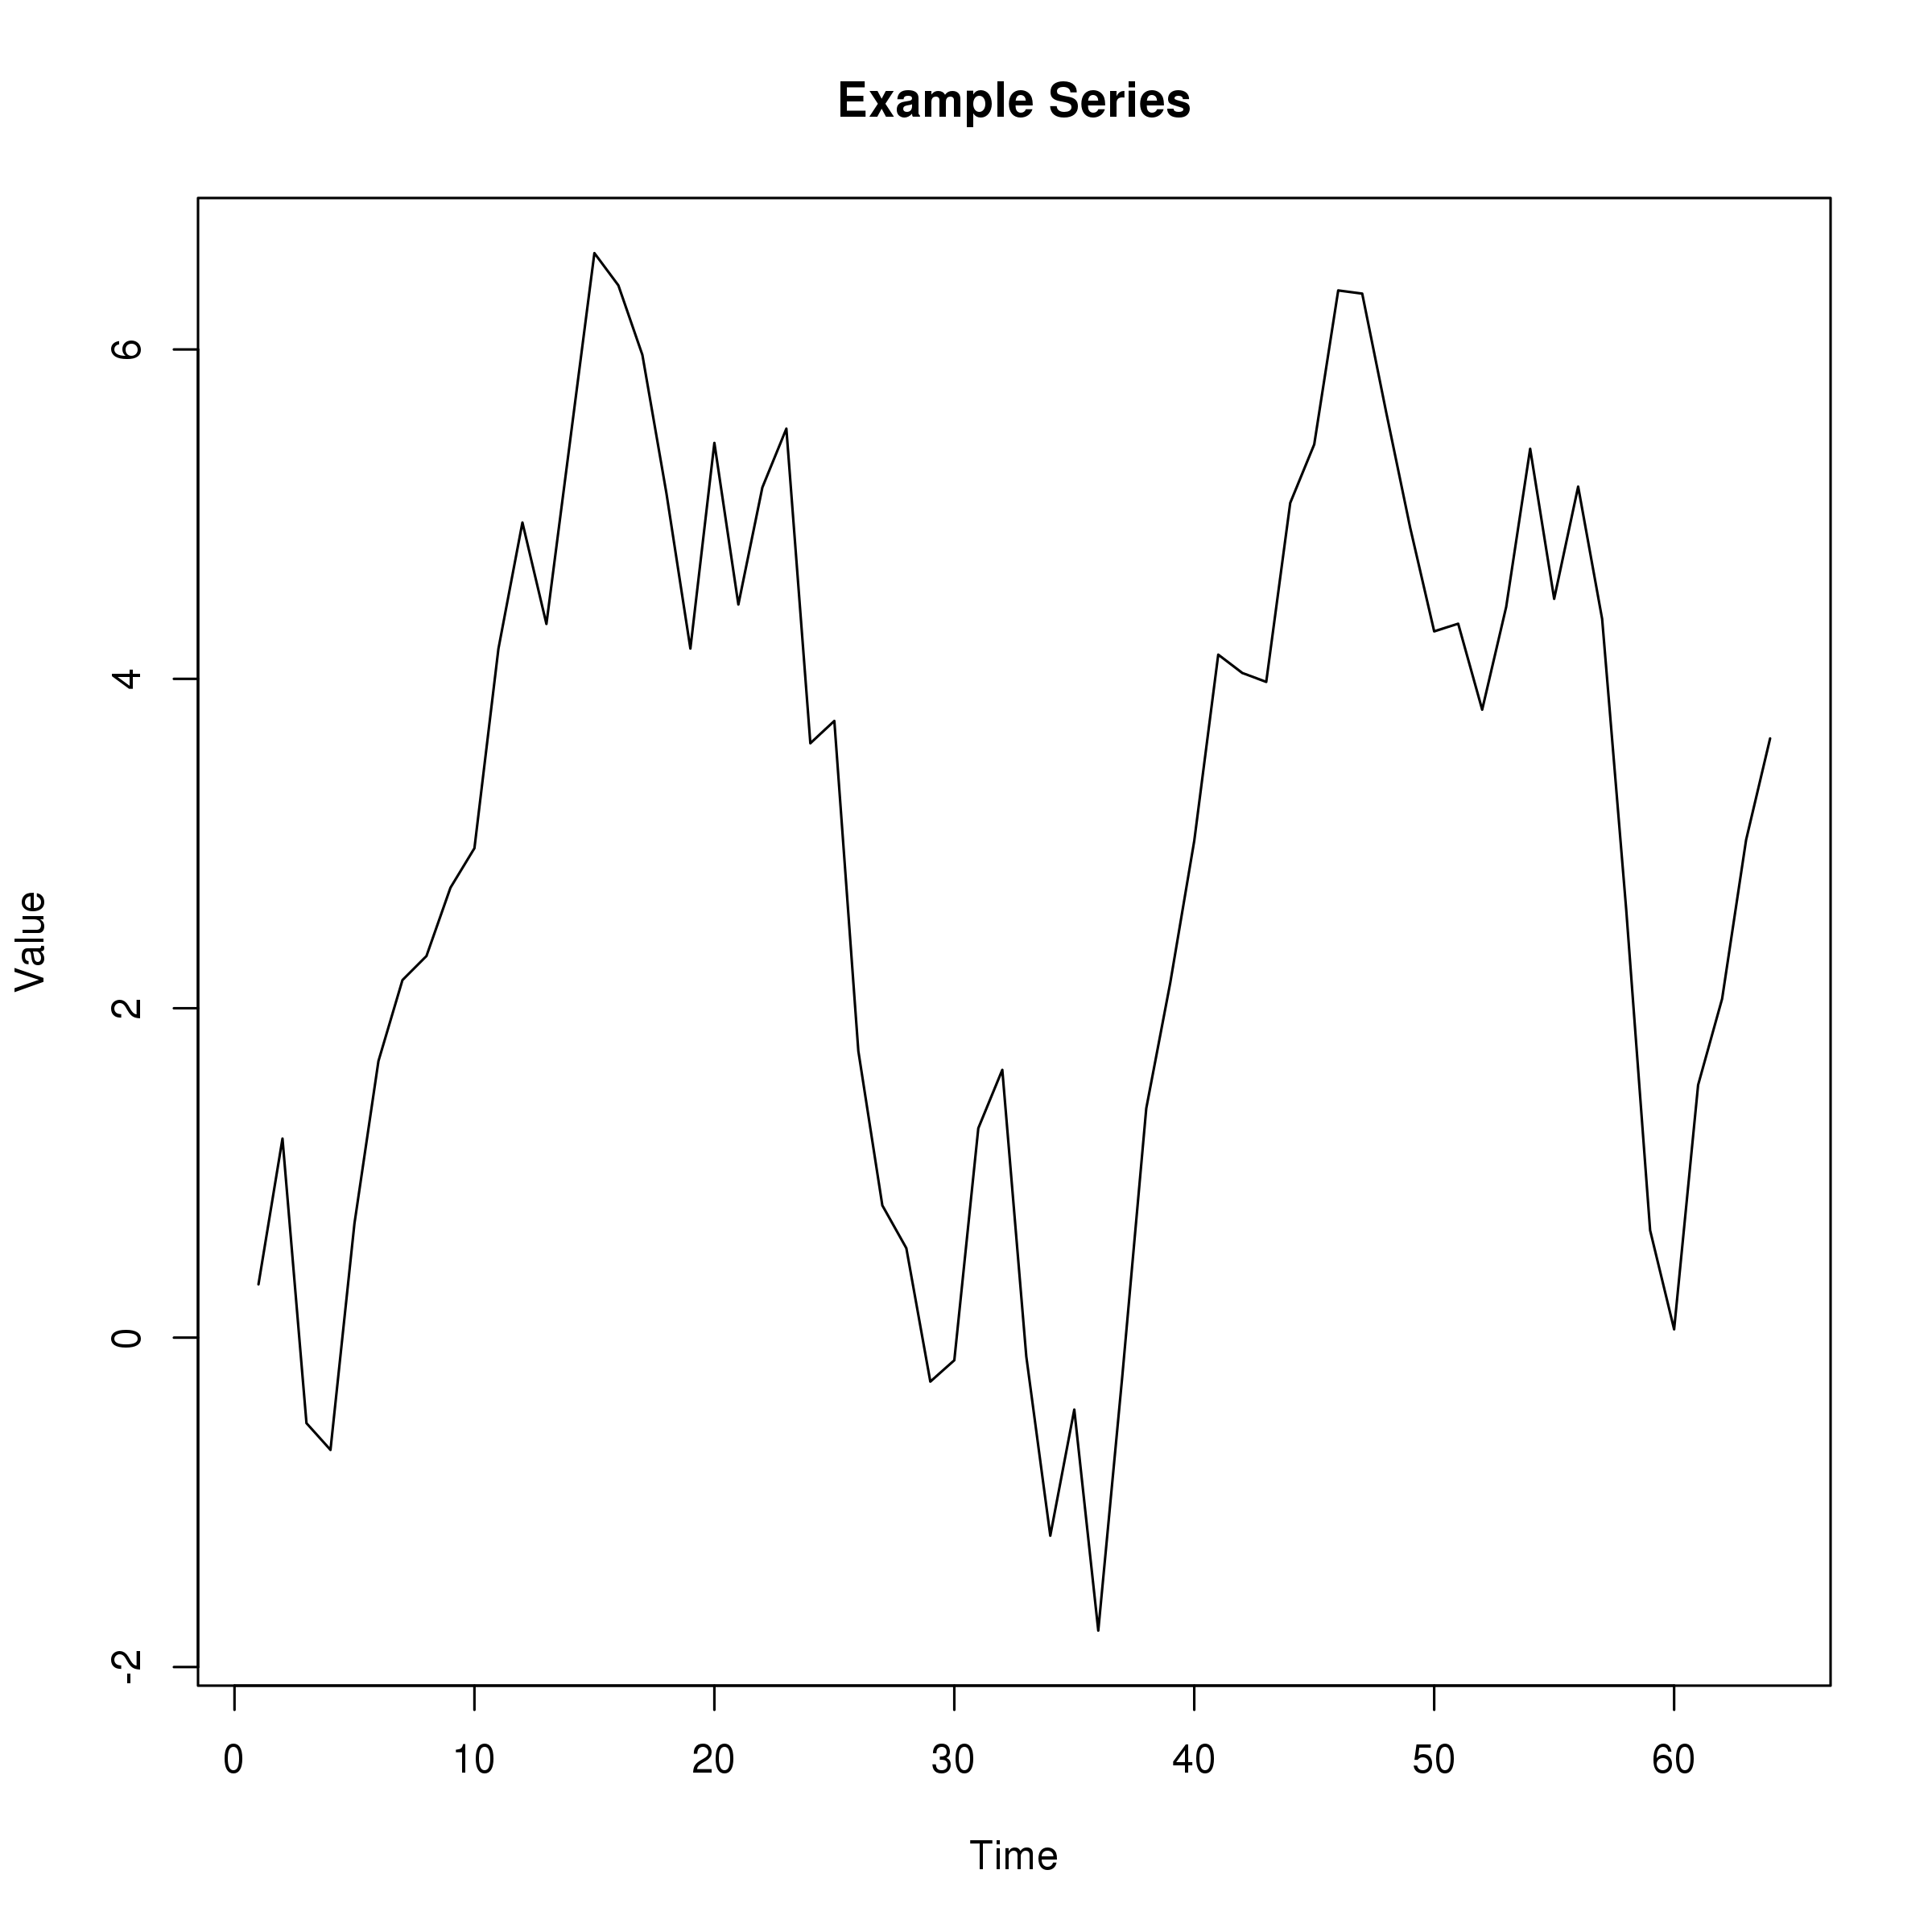
\includegraphics[width = 0.7\textwidth]{res/ex1.png}
    \end{figure}
\end{frame}

\begin{frame}{Practical Details}
\begin{itemize}
    \item
    Computed the periodogram with a $10\%$ Tukey-Hanning taper.
    \item
    Smoothed the log-periodogram using the Epanechnikov kernel
        \[
        K(x) 
        = 
        \frac{3}{4}\pi \biggl[ 1 - \Bigl( \frac{x}{\pi} \Bigr)^2 \biggr].
        \]
    and bandwidth $0.1$ to obtain an estimate of the spectral density.
\end{itemize}
\end{frame}

% Include plots of the Tukey-Hanning taper and the Epanechnikov kernel.

\begin{frame}{Estimator Distribution}
\begin{itemize}
    \item
    Since $\hat{\rho}(1)$ is the Yule-Walker estimate for the AR parameter,
    then as $n \to \infty$,
        \[
        \sqrt{n} \biggl( \frac{\hat{\rho}(1) - 0.9}{\sqrt{c}} \biggr)
        \inD
        \dist{N}(0, 1 - 0.9^2),
        \]
    where $c$ is a correction for the taper.

    \item
    $2000$ bootstrapped estimates (from one simulation)
    produce a bootstrapped distribution.

    \item
    2000 simulations approximate the true distribution.
\end{itemize}
\end{frame}

\begin{frame}{Distributions Plot}
    \begin{figure}
    \centering
    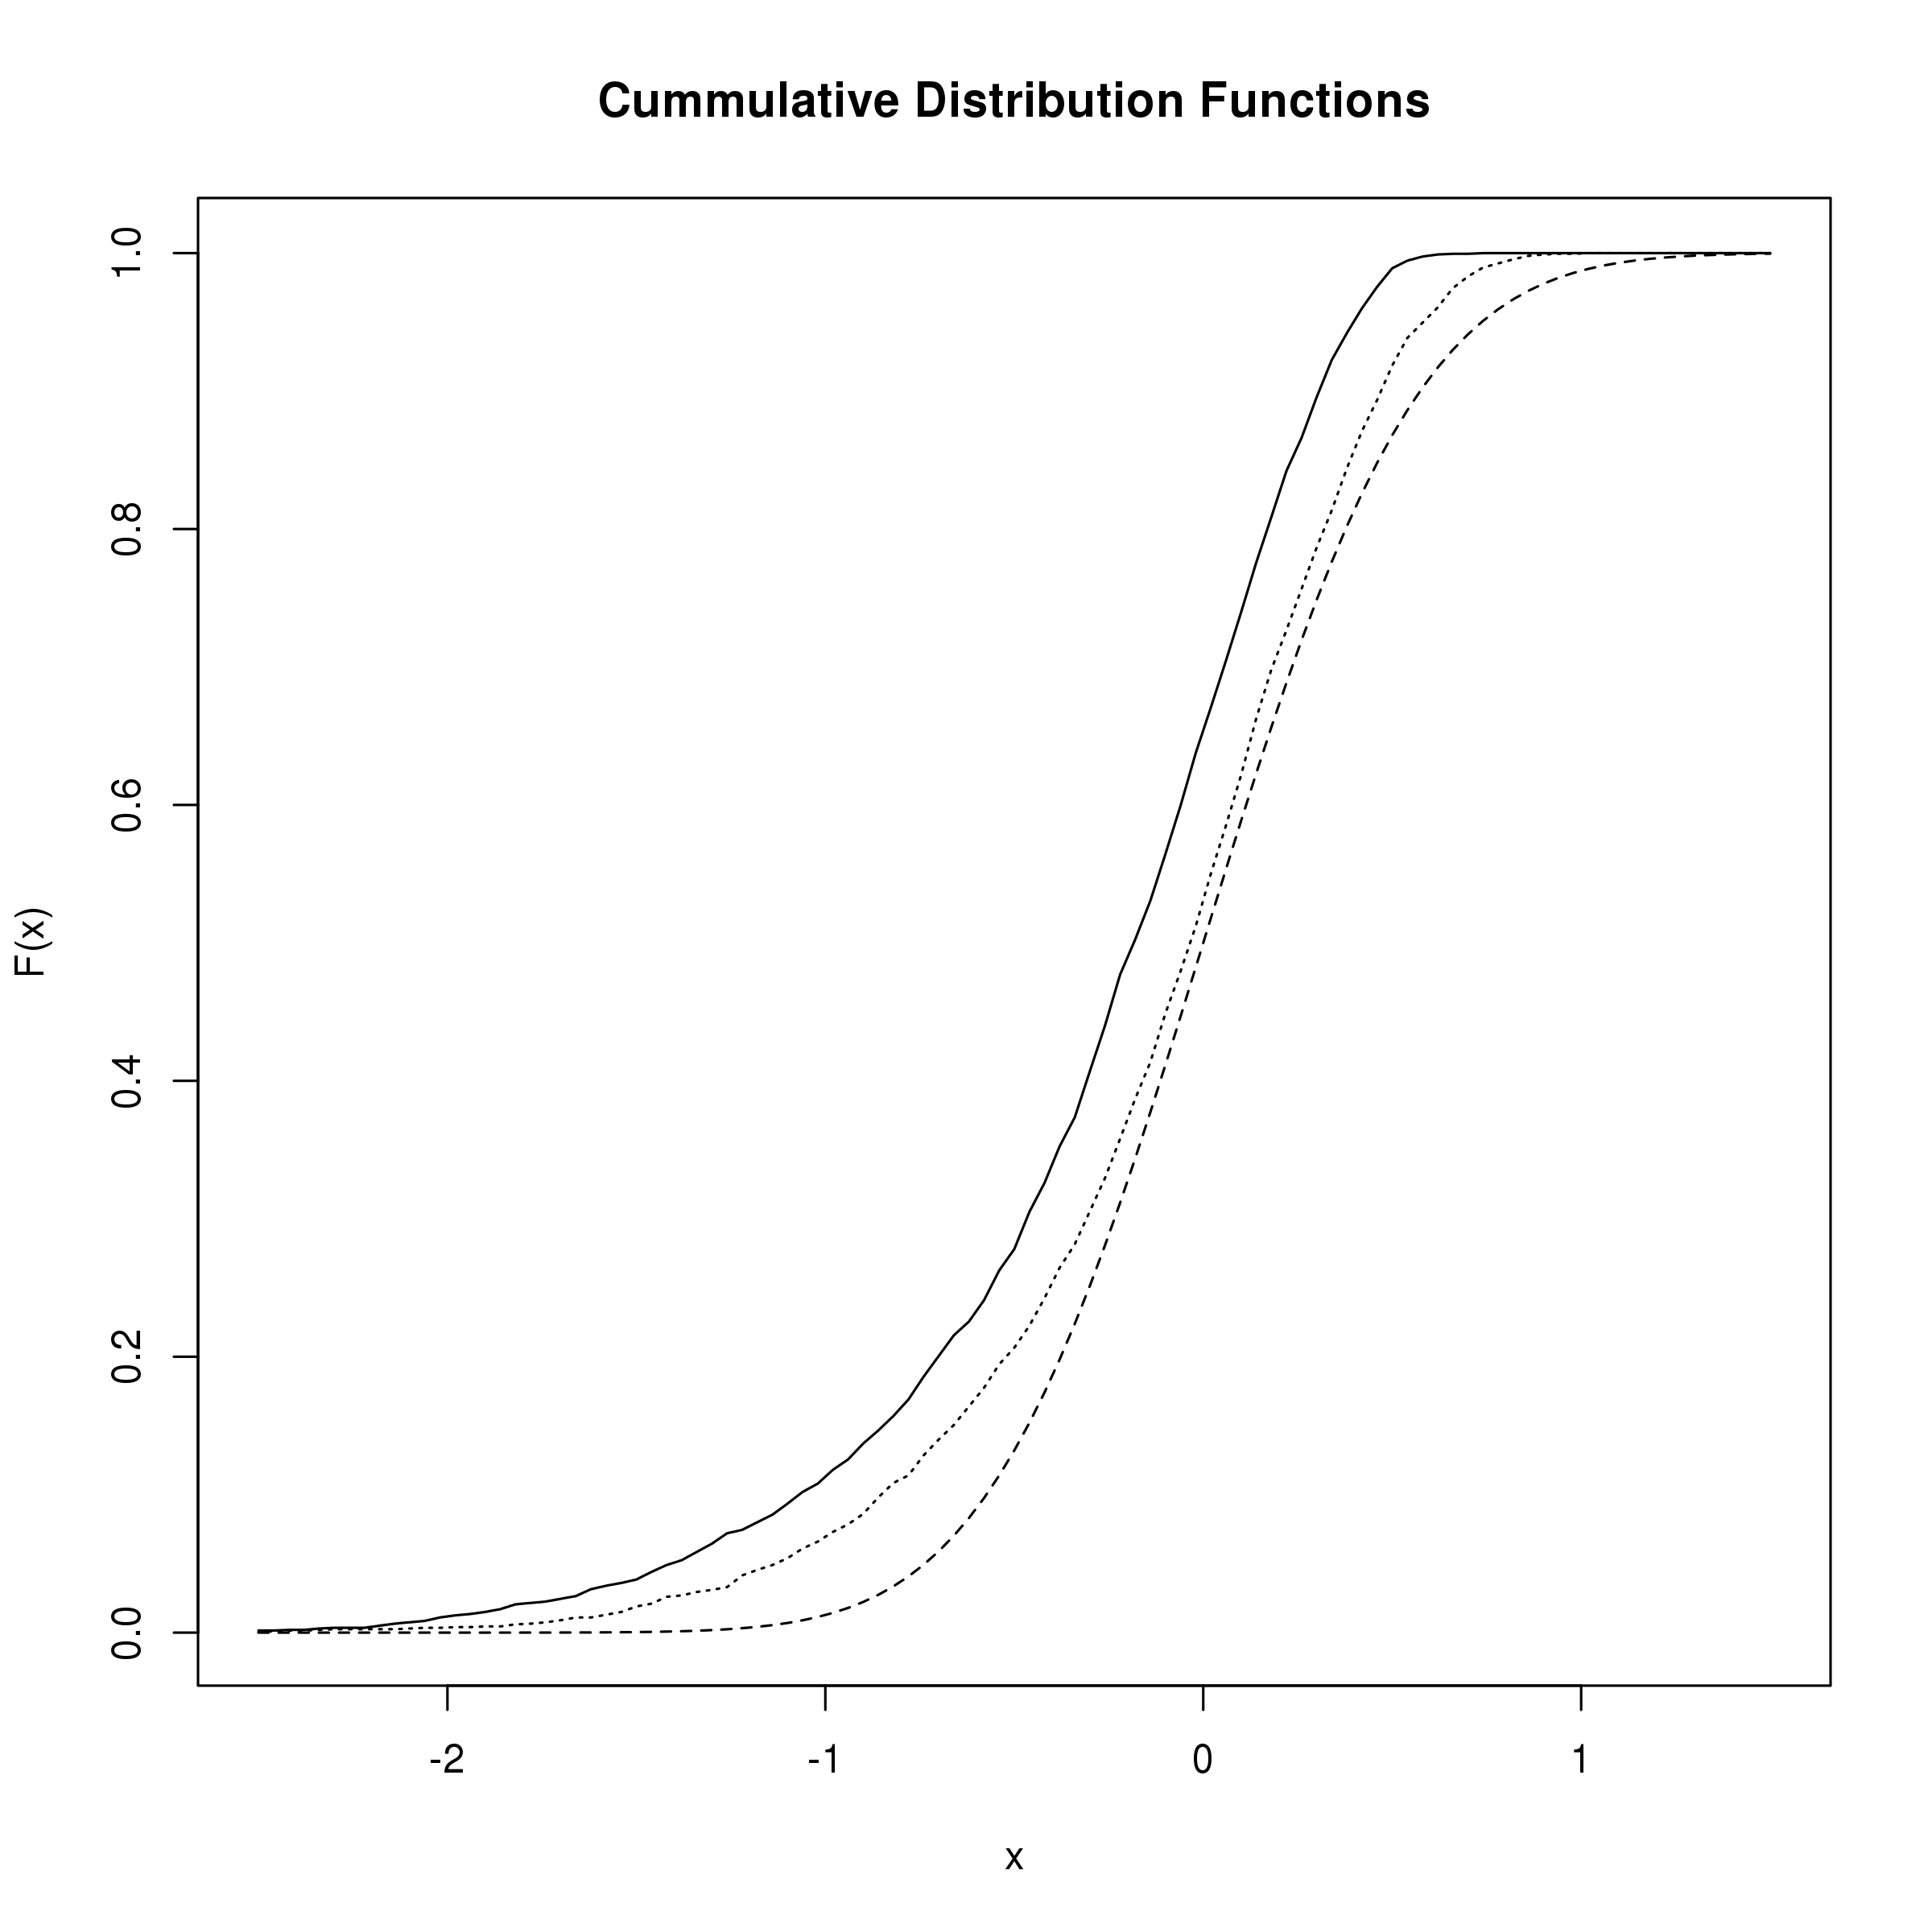
\includegraphics[width = 0.7\textwidth]{res/ex1_cdf.png}
    \end{figure}
\end{frame}

\begin{frame}{Applied Example}
    \begin{figure}
    \centering
    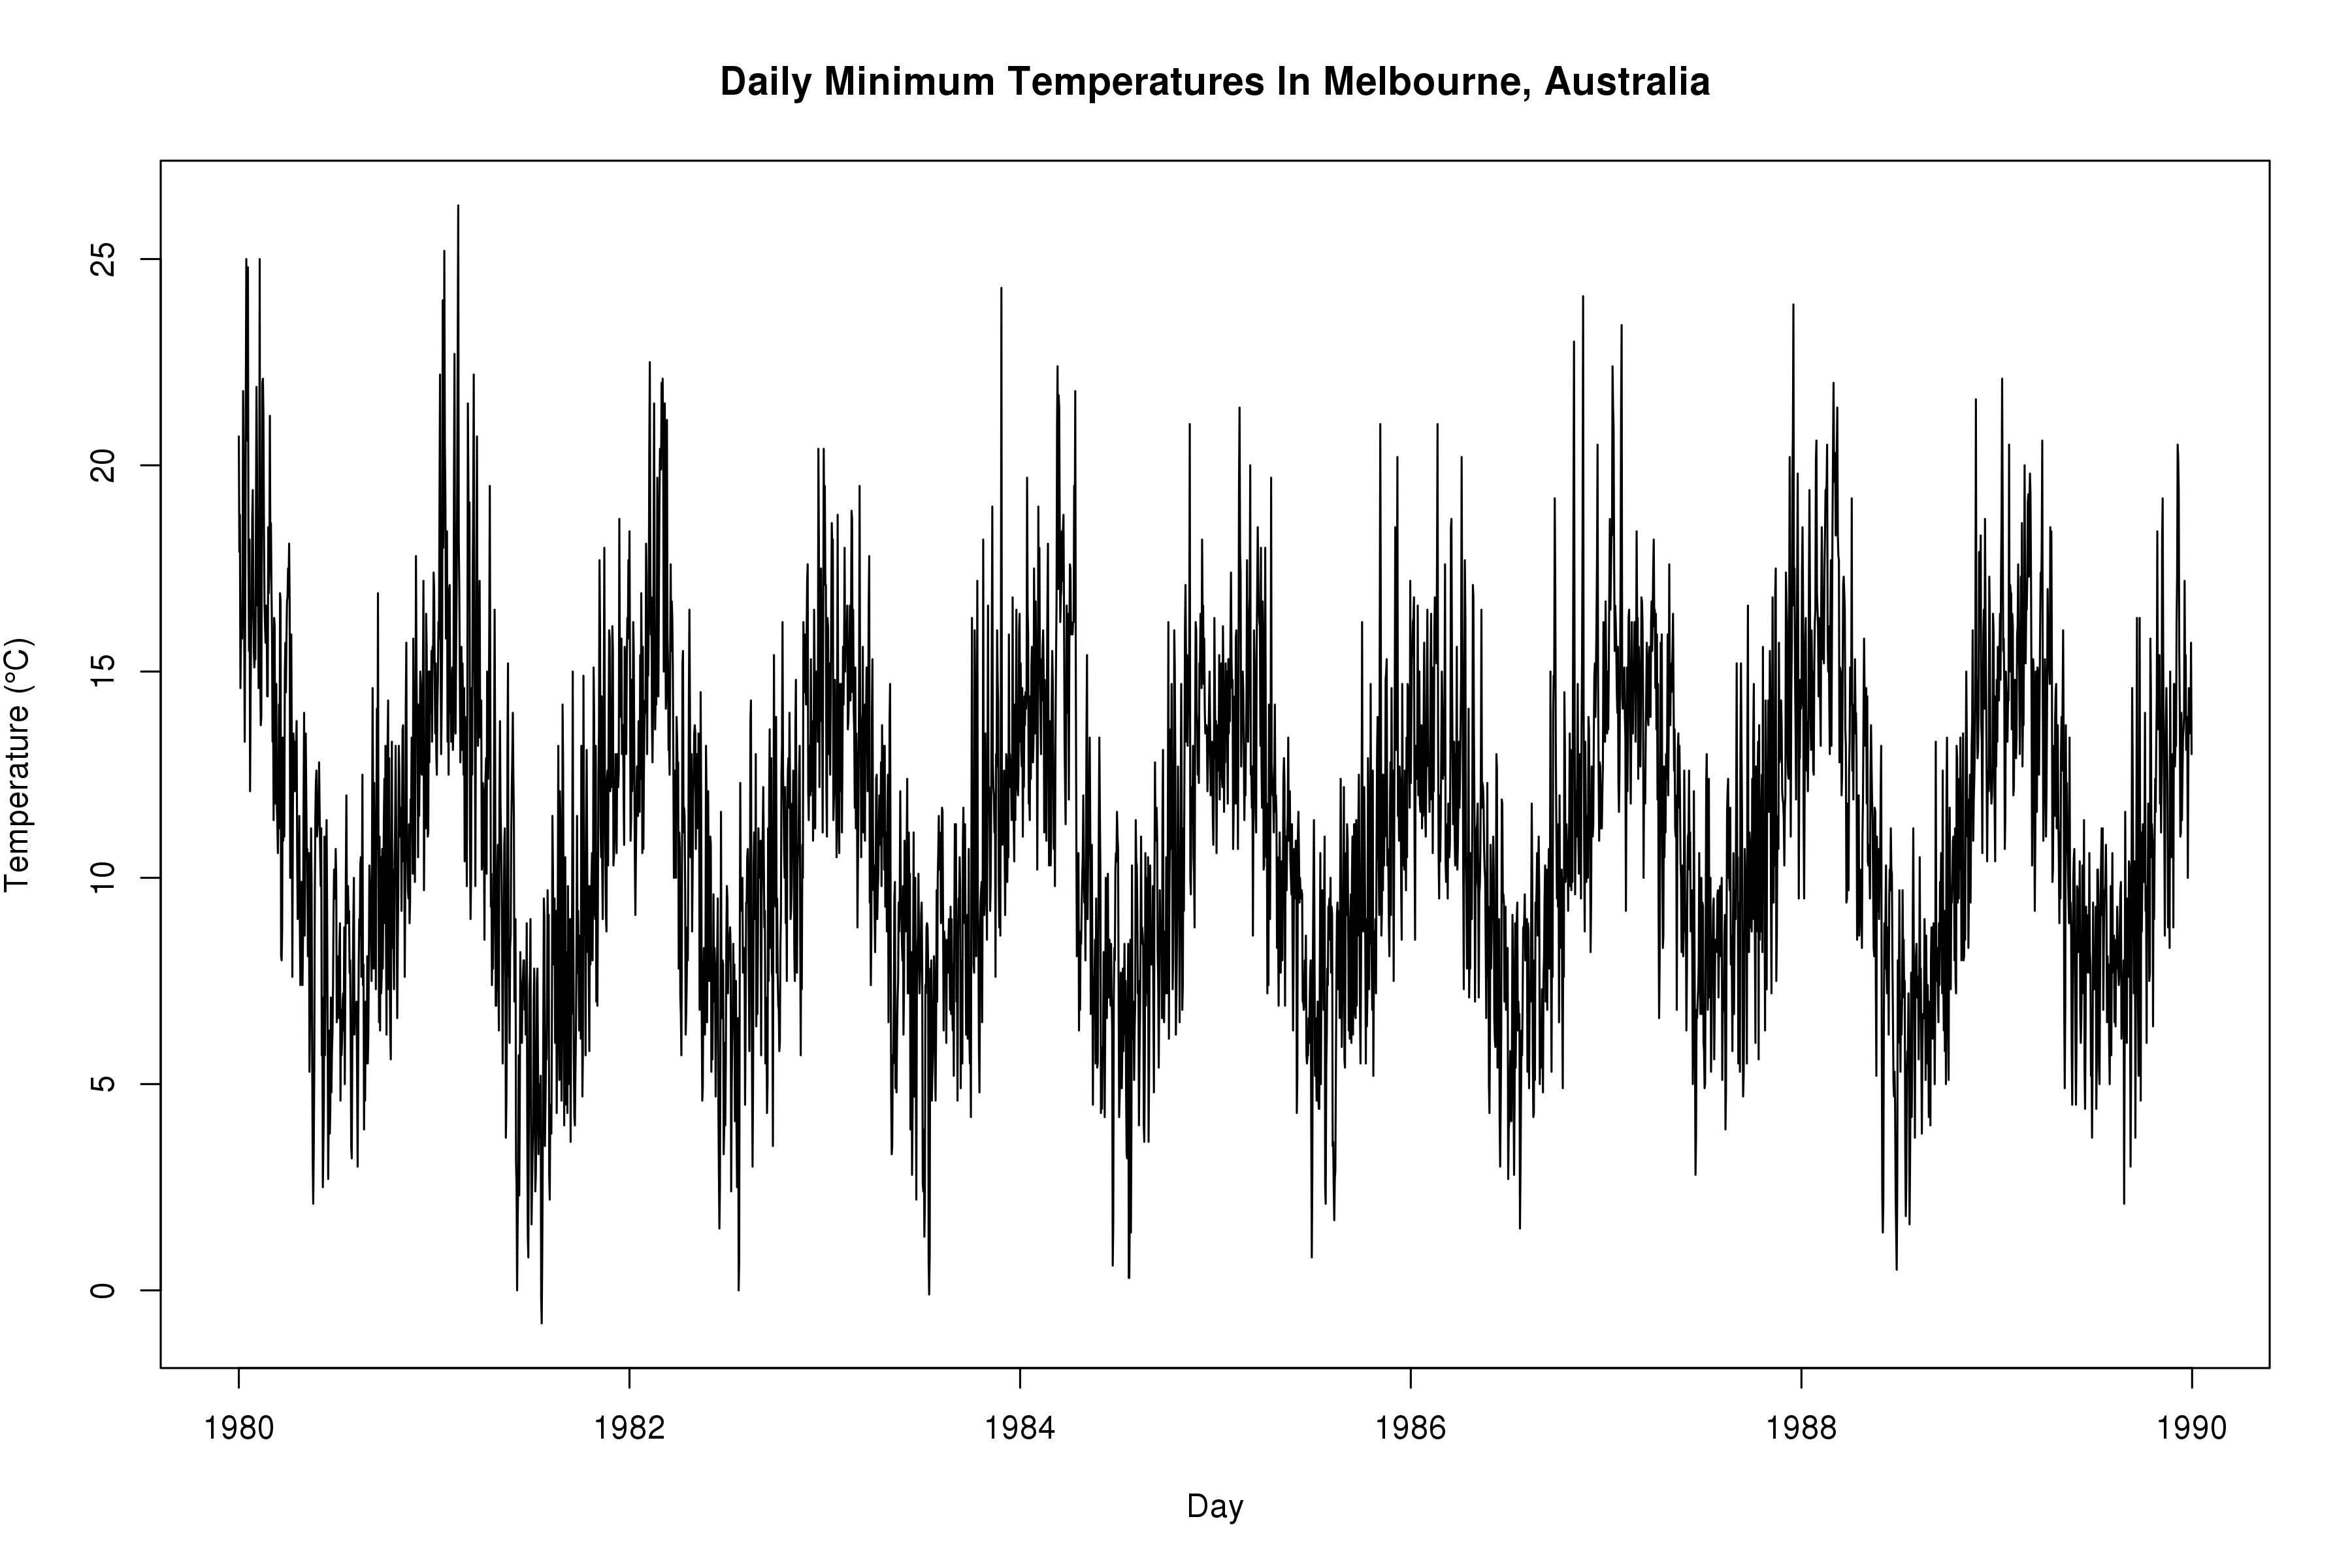
\includegraphics[width = 0.7\textwidth]{res/exA.png}
    \end{figure}
\end{frame}

\begin{frame}{Results}
\end{frame}

 		%uncomment this line to insert your slides
%%%%%%%%%%%%%%%%%%%%%%%%%%%%%%%%%%%

\end{document}
